\documentclass{article}

\usepackage[utf8]{inputenc}
\usepackage[T1]{fontenc}
\usepackage{amssymb}
\usepackage{ntheorem}
\usepackage{amsmath}
\usepackage{multicol}
\usepackage{amssymb}
\usepackage[ a4paper, hmargin={3cm, 3cm}, vmargin={3cm, 3cm}]{geometry}

\usepackage{tikz}
\usetikzlibrary{automata,positioning}

\usepackage{tcolorbox}
\tcbuselibrary{
  theorems,
  breakable,
  skins
}

\usepackage{hyperref}
\hypersetup{
    colorlinks,
    citecolor=black,
    filecolor=black,
    linkcolor=blue,
    urlcolor=blue
}

\newtcbtheorem[number within=section]
{correction}{Correction}{
  colback=white,
  colframe=black!70,
  separator sign none,
  description delimiters parenthesis,
  enhanced jigsaw,
  breakable,
  fonttitle=\bfseries
}{}

\theoremstyle{plain}
\theorembodyfont{\normalfont}
\theoremseparator{~--}
\newtheorem{exercice}{Exercise}[section]

\title{TD n$^\circ$2}
\author{Valeran MAYTIE}
\date{}

\begin{document}
  \maketitle

  \section{Tree automata}

  \exercice Give a bottom-up tree automaton recognizing the language of all
  trees on $\mathcal T(\Sigma)$, with $\Sigma =  \{f^2, g^2, \#\}$ for which the
  following holds:
  \begin{itemize}
    \item a path with symbol $g$ has two children $f$
    \item the root is a $g$
  \end{itemize}

  \begin{correction}{}{}
    Let the automaton $\mathcal A = \{Q = \{q_0, q_1, q_2\}, \Sigma, \delta,
    \{q_2\}\}$ with :

    \[
      \delta = \left \{
        \begin{tabular}{l l r r}
          $\#$          & $\to$ & $q_0$ & \\
          $f(q, q')$    & $\to$ & $q_1$ & $\forall q, q' \in Q$ \\
          $g(q_1, q_1)$ & $\to$ & $q_2$
        \end{tabular}
        \right.
    \]
  \end{correction}

  \exercice Give a bootom-up tree automaton which recognizes all trees over
  $\mathcal(\Sigma)$ with $\Sigma = \{f^2, g^2, \#\}$ with the following shape :

  \begin{center}
    \begin{tikzpicture}
      \node(R)  at ( 0,    0) {$f$};
      \node(G1) at (-1,   -1) {$g$};
      \node(G2) at (-1.5, -2) {$g$};
      \node(G3) at (-2,   -3) {$g$};

      \node(S1) at (-0.5, -2) {$\#$};
      \node(S2) at (-1,   -3) {$\#$};
      \node(S3) at (-1.5, -4) {$\#$};
      \node(S4) at (-2.5, -4) {$\#$};

      \draw (G1) -- (S1) (G2) -- (S2) (G3) -- (S3) (G3) -- (S4);
      \draw (R) -- (G1) (G2) -- (G3);
      \draw[dashed] (G1) -- (G2);

      \node(S1) at (0.5, -2) {$\#$};
      \node(S2) at (1,   -3) {$\#$};
      \node(S3) at (1.5, -4) {$\#$};
      \node(S4) at (2.5, -4) {$\#$};
      \node(F1) at (1,   -1) {$f$};
      \node(F2) at (1.5, -2) {$f$};
      \node(F3) at (2,   -3) {$f$};

      \draw (R) -- (F1) (F2) -- (F3);
      \draw[dashed] (F1) -- (F2);
      \draw (F1) -- (S1) (F2) -- (S2) (F3) -- (S3) (F3) -- (S4);
    \end{tikzpicture}
  \end{center}

  \begin{correction}{}{}
    Let the automaton
    $\mathcal A = \{Q=\{q_0, q_1, q_2, q_3\}, \Sigma, \delta, \{q_3\}\}$ with :
    \[
      \delta = \left \{
        \begin{tabular}{l l r l l l r l}
          $\#$          & $\to$ & $q_0$ \\
          $f(q_0, q_0)$ & $\to$ & $q_1$ & $g(q_0, q_0)$ & $\to$ & $q_2$ \\
          $f(q_0, q_1)$ & $\to$ & $q_1$ & $g(q_2, q_0)$ & $\to$ & $q_2$ \\
          $f(q_2, q_2)$ & $\to$ & $q_3$ \\
        \end{tabular}
        \right.
    \]
  \end{correction}

  \exercice Let $\Sigma ) \{+^2, \times^2, a, b\}$, consider the language on
  $\Sigma$ of non ambiguous arithmetic expressions (that is, expressions which
  do not require parenthesis). For instance the tree :

  \begin{center}
    \begin{tikzpicture}
      \node(+)  at ( 0.0, 0  ) {$+$};
      \node(a1) at (-0.5,-0.75) {$a$};
      \node(x)  at ( 0.5,-0.75) {$\times$};
      \node(a2) at ( 0,  -1.5 ) {$a$};
      \node(b)  at ( 1,  -1.5 ) {$b$};

      \draw (+) -- (a1) (+) -- (x) -- (a2) (x) -- (b);
    \end{tikzpicture}
  \end{center}

  is non ambiguous. Is this language regular ? Is it top-down recognizable ?

  \begin{correction}{}{}
    Let the top-down automaton $\mathcal A = \{\{q_0, q_1\}, \Sigma, \delta,
    \{q_0\}\}$ with :
    \[
      \delta = \left \{
        \begin{tabular}{l l l l l l}
          $q_0, a$ & $\to$ & $\{\}$ & $q_0, b$ & $\to$ & $\{\}$ \\
          $q_1, a$ & $\to$ & $\{\}$ & $q_1, b$ & $\to$ & $\{\}$ \\
          \\
          $q_0, \times$ & $\to$ & $\{(q_1, q_1)\}$ &
          $q_0, +$      & $\to$ & $\{(q_0, q_0)\}$ \\
          $q_1, \times$ & $\to$ & $\{(q_1, q_1)\}$ \\
        \end{tabular}
        \right.
    \]

    An expression is non ambiguous, if below the $\times$ there are only
    $\times$ or constants $(a, b)$. We have a top-down regular automaton so
    this language is regular.
  \end{correction}

  \exercice Let $T$ be a tree language. Define $\textit{leaves}(t)$ as the word
  formed by taking all the symbols with arity 0 encountered during a depth
  first, left to right traversal of the tree. Formally, such a word can be
  written as the longest sequence of symbols : $t(l_1), t(l_2), \ldots, t(l_k)$
  for which the following hold :
  \begin{itemize}
    \item $\forall i, |t(l_i)| = 0$
    \item $\forall i, j, i < j \Rightarrow l_i <_{\text{lex}} l_j$
      ($<_{\text{lex}}$ : the lexicographic order on paths).
  \end{itemize}
  We define $\textit{leaves}(T) = \{\textit{leaves}(t) | t \in T\}$. Show that
  even in the case where $T$ is a recognizable tree language,
  $\textit{leaves}(T)$ is not necessarily a regular word language.
 
  \begin{correction}{}{}
    We can consider the language $\mathcal T$ :

    \begin{align*}
      l(\texttt (, \texttt ), t) &\in \mathcal T \\
      r(\texttt (, t, \texttt )) &\in \mathcal T \\
      n(\texttt (, \texttt )) &\in \mathcal T \\
    \end{align*}

    $\mathcal T$ is a tree language recognized by
    $\mathcal A =\{\{q_0, q_1, q_2\}, \Sigma = \{l^3, r^3, n^2, \texttt (,
    \texttt)\}, \delta, \{q_2\}\}$ with :

    \[
      \delta = \left \{
        \begin{tabular}{l l l l l l}
          $\texttt ($   & $\to$ & $q_0$ & $\texttt )$        & $\to$ & $q_1$ \\
          $n(q_0, q_1)$ & $\to$ & $q_2$ & $r(q_0, q_2, q_1)$ & $\to$ & $q_2$ \\
          $l(q_0, q_1, q_2)$ & $\to$ & $q_2$ \\
        \end{tabular}
        \right.
    \]

    The language $\textit{leaves}(T)$ represent the Dyck's word. But this
    language is not regular.
  \end{correction}

  \newpage
  \exercice Show that the set of perfect binary trees over $\Sigma = \{f^2, a\}$
  is not regular. A prefect binary tree is a tree for which all leaves have the
  same depth (that is, all paths to leafs have the same length).

  \begin{correction}{}{}
    We suppose that this language $\mathcal T$ is regular. So by the pumping
    lemma we have a $p \geq 1$ such that for all $t \in \mathcal T$ of
    $\texttt{height}(t) \geq p$, there exists $C$, $C' \in \mathcal T(\Sigma,
    \{\square\})$ with $C'$ non trivial and
    $u \in \mathcal T$ such that $t =C[C'[u]]$ and for all
    $n\geq 0$, $C[C'^n[u]] \in \mathcal T$.
    
    $C'$ is non trivial (it can not be $\square$) so it contains at least one
    $f$ :

    \begin{center}
      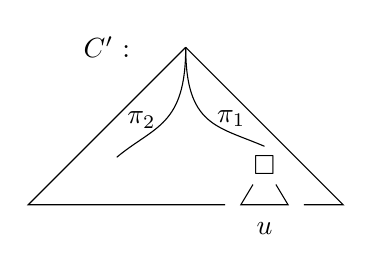
\begin{tikzpicture}
        \node at (-1, 0) {$C'$ :};
        \node(S1) at (-1, -1.5) {};
        \node(S2) at ( 1, -1.5) {$\square$};
        \draw (0, 0) -- (-2, -2) -- (0.5, -2) (1.5, -2) -- (2, -2) -- (0, 0);

        \draw (0, 0) .. controls (0,-1) and (0.4, -1) ..
              node[right]{$\pi_1$}(S2.90);
        \draw (0, 0) .. controls (0,-1) and (-0.4, -1) ..
              node[left]{$\pi_2$}(S1);

          \draw (S2) -- (1.3, -2) -- (0.7, -2)  -- (S2);
        \node at (1, -2.3) {$u$};
      \end{tikzpicture}
    \end{center}

    $C'[u]$ is perfect so the height of the tree on $\pi_1$ and $\pi_2$ are
    equals. But if we consider the tree $C'[C'[u]]$
    the height of the tree on $\pi_1$ and $\pi_2$ are different :

    \begin{center}
      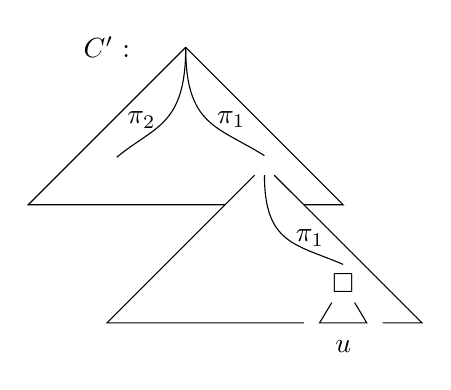
\begin{tikzpicture}
        \node at (-1, 0) {$C'$ :};
        \node(S1) at (-1, -1.5) {};
        \node(S2) at ( 1, -1.5) {};

        \draw (0, 0) -- (-2, -2) -- (0.5, -2) (1.5, -2) -- (2, -2) -- (0, 0);
        \draw (S2) -- (-1, -3.5) -- (1.5, -3.5) (2.5, -3.5) -- (3, -3.5) -- (S2);


        \draw (0, 0) .. controls (0,-1) and (0.4, -1) ..
              node[right]{$\pi_1$}(S2.90);
        \draw (0, 0) .. controls (0,-1) and (-0.4, -1) ..
              node[left]{$\pi_2$}(S1);

        \node(S) at ( 2, -3) {$\square$};
        \draw (S2) .. controls (1,-2.5) and (1.4, -2.5) ..
          node[right]{$\pi_1$}(S.90);

        \draw (S) -- (1.7, -3.5) -- (2.3, -3.5)  -- (S);
        \node at (2, -3.8) {$u$};
      \end{tikzpicture}
    \end{center}

    $C[C'^2[u]] \not \in \mathcal T$ which contradicts the pumping lemma. So the
    language $\mathcal T$ is not regular.
  \end{correction}

  \exercice Let $\mathcal T$ be a language over $\Sigma =\{f^2, a, b\}$.
  Consider the congruence $f(x, y) \equiv f(y, x)$ for $x, y \in \mathcal
  T(\Sigma)$. Show that if $\mathcal T$ is regular, the set
  $\mathcal T' = \{t' | \exists t \in T, t \equiv t'\}$ is regular.

  \begin{correction}{}{}
    Let $\mathcal A = \{Q, \Sigma, \delta, \mathcal I\}$ a top-down tree
    automaton who recognizes the language $\mathcal T$.

    We can construct a top-down tree automaton which recognizes the language
    $\mathcal T'$:

    \vspace{5mm}

    $\mathcal A' = \{Q, \Sigma, \delta', \mathcal I\}$ with :
    \[
      \delta' = \left \{
        \begin{tabular}{l l l}
          $a$ & $\to$ & $\delta(a)$ \\
          $b$ & $\to$ & $\delta(b)$ \\
          $f(q, q')$ & $\to$ & $\delta(f(q', q))$ \\
        \end{tabular}
        \right.
    \]
  \end{correction}
 
\end{document}
